





\documentclass[12pt, a4paper]{report}






%-----------USEPACKAGE----------------------------
\usepackage{bm} % Tucne pismo
\usepackage[czech]{babel} % Cestina
\usepackage[T1]{fontenc}
\usepackage[utf8x]{inputenc}
\usepackage[unicode]{hyperref} % Odkazy v pdf, www a na e-mail
\usepackage{graphicx} % Obrazky
\usepackage{epstopdf} % Obrazky
\linespread{1.10} % Radkovani 1.3 odpovida radkovani 2
\usepackage{lmodern} % Daji se pouzit \HUGE atd.
\usepackage{amsmath}
\usepackage{algorithm}
\usepackage[noend]{algpseudocode} % Vkladani pseudo kodu

\usepackage[numbered,framed]{matlab-prettifier} %vkladani kodu matlabu
\lstset{style = Matlab-editor, basicstyle = \mlttfamily, escapechar = ", mlshowsectionrules = true,}








%------------------DRAFT----------------------------
\usepackage{draftwatermark}
\SetWatermarkLightness{0.95}
\SetWatermarkScale{1}
\SetWatermarkText{DRAFT}











%------------------LAYOUT----------------------------
\usepackage[top = 2.5 cm, bottom = 2.5 cm, left = 2.5 cm, right = 2.5 cm]{geometry} % geometrie stranky
\usepackage{longtable}% Pro dlouhy obsah, da se zalomit \pagebrek
\usepackage{fancyhdr}
\pagestyle{fancy}% Deffaultni nastaveni hlavicky a paticky
\setlength{\headheight}{16 pt}% Zvetsi hlavicku, aby to nedelalo warningy
\fancyhf{}
\lhead{\href{http://www.kky.zcu.cz/cs/courses/mpv}{Metody Počítačového Vidění}}
\rhead{8. přednáška}
\fancyfoot[R]{\thepage}
\fancyfoot[L]{Verze 1.0.0, poslední úpravy: \today}








\begin{document}








%--------TITULNI-STRANA------------------------------
\begin{titlepage}
\begin{center}
	
\includegraphics[trim = 0.6cm 0.5cm 0.9cm 0.5cm, scale=1]{./Img/FAV_logo_cz.pdf}
	\hspace*{\fill}
	
\includegraphics[trim = 3.5cm 1.5cm 2.6cm 2cm, scale=0.295]{./Img/KKY_logo_cz.pdf}\\
	\vspace*{\fill}
	\textbf{\Huge{\href{http://www.kky.zcu.cz/cs/courses/mpv}{Metody Počítačového Vidění} \\ 9. přednáška: Strojové učení}}\\
	\vspace*{\fill}
	\textbf{\large{\href{mailto:LBures@kky.zcu.cz}{Ing. Lukáš Bureš}}} \hfill ~\\
	\textbf{\large{\href{mailto:PetrZim@kky.zcu.cz}{Ing. Petr Zimmermann}}} \hfill \textbf{\large{Plzeň}}\\
	\textbf{\large{Katedra kybernetiky}} \hfill \textbf{\large{\today}}
\end{center}
\end{titlepage}









%--------OBSAH----------------------------------------
\setcounter{page}{1}
\pagenumbering{Roman}

\tableofcontents
\newpage

\setcounter{page}{1}
\pagenumbering{arabic}








%--------SEKCE----------------------------------------





%----PREDNASKA-09--------------------------------------------------------------------------
\chapter{Metody Počítačového Vidění 9.~přednáška}










%----BAYESOVSKA-KLASIFIKACE--------------------------------------------------------------
\section{Bayesovská klasifikace}
\par{Bayesovská rozhodovací teorie je základní statistický přístup ke klasifikaci. Tento přístup je založen na vyčíslení kompromisu mezi různými klasifikačními rozhodnutími za využití pravděpodobnosti a nákladů, které doprovázejí rozhodnutí. Za předpokladu, že problém rozhodování je představen pomocí pravděpodobnostních vztahů, kde jsou všechny hodnoty pravděpodobností známé.}

\par{Označme $\omega$ (\textit{přirozený stav}) jednotlivé třídy, do kterých budeme klasifikovat. Při klasifikaci do dvou tříd mějme $\omega_1$ a $\omega_2$, tedy $\omega = \omega_1$ a $\omega = \omega_2$. Protože \textit{přirozený stav} je nepredikovatelný, považujme $\omega$ za proměnou, která musí být popsána pravděpodobnostně.}

\par{Předpokládejme, že tu je nějaká \textit{apriorní} pravděpodobnost $P(\omega_1)$, taková, že vzorek patří do třídy $\omega_1$ a $P(\omega_2)$ do třídy $\omega_2$. Dále předpokládejme, že neexistují žádné další třídy, proto $P(\omega_1) + P(\omega_2) = 1$. Tato \textit{apriorní} znalost reflektuje jaké je pravděpodobnost, že vzorek bude patřit do třídy $\omega_1$ nebo $\omega_2$, ještě dříve než se vzorek zobrazí.}

\par{Předpokládejme pro tuto chvíli, že chceme rozhodnout do jaké třídy vzorek patří bez jeho pozorování. Jediná informace, kterou je možné využít je \textit{apriorní} pravděpodobnost. Pokud musí být učiněno rozhodnutí s takto malou informací, zdá se logické použít následující rozhodovací pravidlo: vzorek patří do třídy $\omega_1$ pokud $P(\omega_1) > P(\omega_2)$, jinak patří do třídy $\omega_2$.}

\par{Ve většině případů nejsme nuceni nejsme nuceni učinit rozhodnutí pouze na základě \textit{apriorní} pravděpodobnosti. Uvažujme $x$, jako spojitou náhodou veličinu, jejíž distribuce závisí na \textit{přirozeném stavu} a je vyjádřená jako $p(x|\omega_1)$, což je podmíněná hustota pravděpodobnosti třídy $\omega_1$. Přesněji lze podmíněnou hustotu pravděpodobnosti $p(x|\omega_1)$ zapsat jako $p_X (x|\omega_1)$, což naznačuje, že se jedná zejména o náhodnou proměnnou $X$. Tedy, pro upřesnění, v případě $p_X(\cdot)$ a $p_Y(\cdot)$ se jedná o dvě různé funkce, které můžeme zapsat jako $p(x)$ a $p(y)$. Rozdíl mezi $p(x|\omega_1)$ a $p(x|\omega_2)$ popisuje rozdíl mezi jednotlivými třídami, viz Obr. \ref{fig:bayes}.} 

\begin{figure}[!ht]
	\centering
	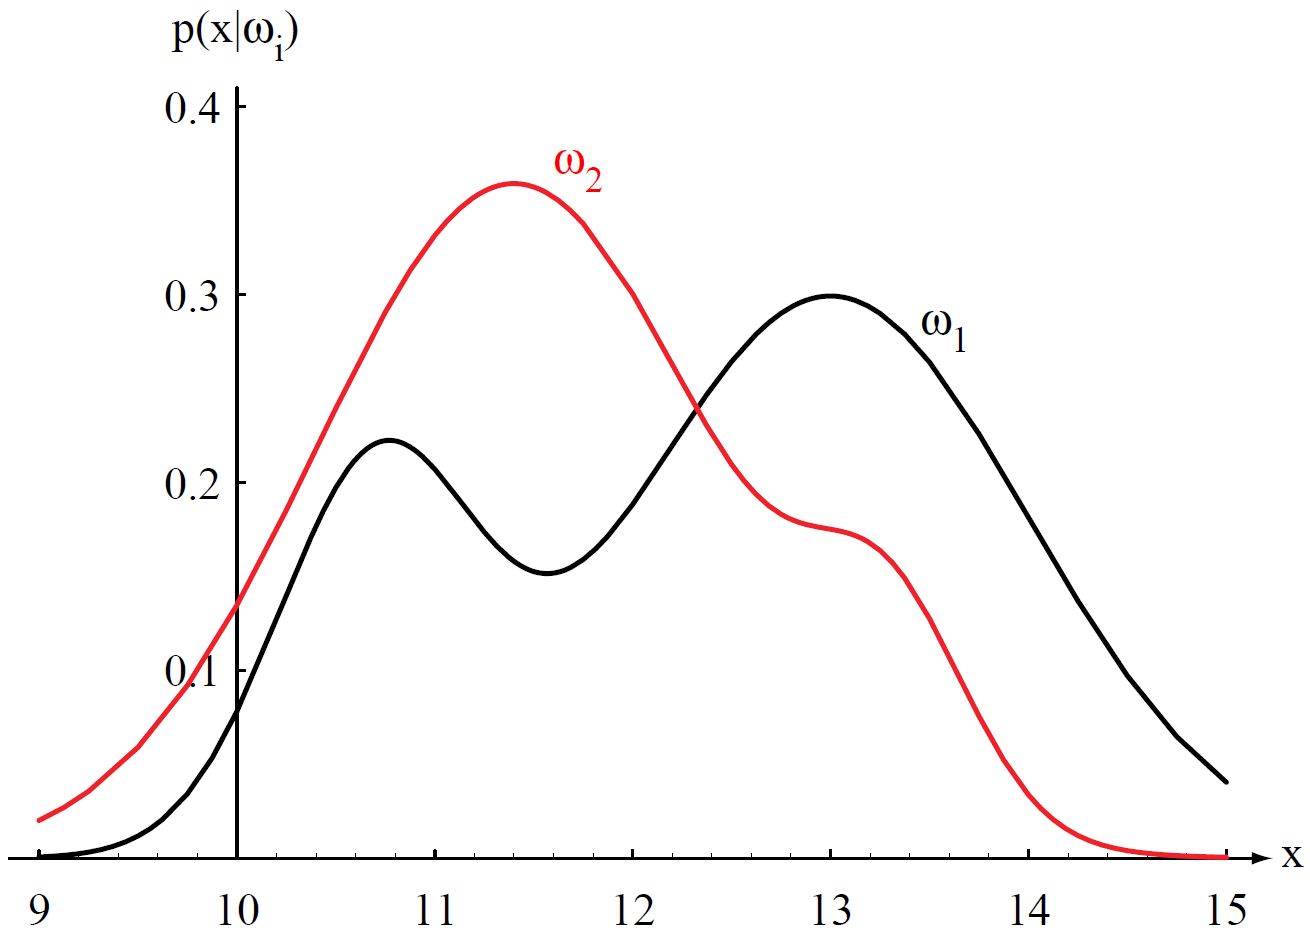
\includegraphics[width = 0.6\textwidth]{./Img/Prednaska09/bayes/bayes.png}
	\caption{Hypotetické funkce hustot podmíněných pravděpodobností ukazují hustotu pravděpodobnosti měření hodnoty příznaku $x$ za předpokladu, že vzorek náleží třídě $\omega_i$. Hustotní funkce jsou normalizované a plocha pod každou křivkou má obsah roven 1.}
	\label{fig:bayes}
\end{figure}
\pagebreak

\par{Předpokládejme, že známe apriorní pravděpodobnosti $P(\omega_j)$ a podmíněné závislosti $p(x|\omega_j)$. Spojitá hustota pravděpodobnosti, že vzorek patří do třídy $\omega_j$ a má hodnotu příznaku $x$ a může být zapsáno dvěma způsoby: $p(\omega_j, x) = P(\omega_j|x) p(x) = p(x|\omega_j)P(\omega_j)$, přeuspořádáním tohoto vztahu dostaneme známý Bayesův vztah
\begin{equation}
	P(\omega_j|x) = \frac{p(x|\omega_j) P(\omega_j)}{p(x)},
\end{equation}
kde v případě dvou tříd
\begin{equation}
	p(x) = \sum_{j = 1}^2 p(x|\omega_j) P(\omega_j)
\end{equation}}

\par{Bayesův vztah může být vyjádřen slovně jako
\begin{equation}
	\mbox{posterior} = \frac{\mbox{likelihood} \times \mbox{prior}}{\mbox{evidence}}.
\end{equation}}

\par{Bayesův vztah ukazuje, že pozorováním hodnoty $x$ můžeme konvertovat apriorní pravděpodobnost $P(\omega_j)$ na aposteriorní pravděpodobnost $P(\omega_j|x)$ - pravděpodobnost přirozeného stavu $\omega_j$ je dána pozorovanou hodnotou $x$.}





\newpage















%----ROZHODOVACI-STROM-------------------------------------------------------------------
\section{Rozhodovací strom}
\label{sec:DecisionTree}
\par{Rozhodovací strom je příkladem nelineární klasifikační metody. Představuje vícepatrový rozhodovací systém, kterým příznakové vektory postupně procházejí až do bodu, kdy jsou zařazeny do odpovídající třídy.}

\par{Sestavení rozhodovacího stromu se provádí postupným dělením prostoru trénovací množiny $X$ na navzájem se neprolínající regiony, přičemž každý region odpovídá právě jedné klasifikační třídě. Rozhodovací strom $T$ se skládá z uzlů, uvnitř kterých dochází k~porovnávání jednotlivých prvků příznakového vektoru $\bm{x}\in X$. Na základě těchto porovnání vektor postupně propadne až do jednoho z listů stromu, které odpovídají jednotlivým klasifikačním třídám. Obecně nejpoužívanější forma rozhodovacího stromu je ta, která rozděluje prostor vstupní množiny na kvádry, jejichž hrany jsou rovnoběžné se souřadnicovými osami tohoto prostoru. Takový strom se nazývá stromem binárním a prvky příznakového vektoru jsou porovnávány na základě splnění nerovnosti $x_i \leq\alpha$, kde $x_i$ je $i$-tý prvek příznakového vektoru $\bm{x}$ a $\alpha$ značí zvolený práh. Nerovnost $x_i \leq\alpha$ je označována jako rozhodovací pravidlo.
\begin{figure}[!ht]
	\centering
	%trim option's parameter order: left bottom right top
	%\fbox{
	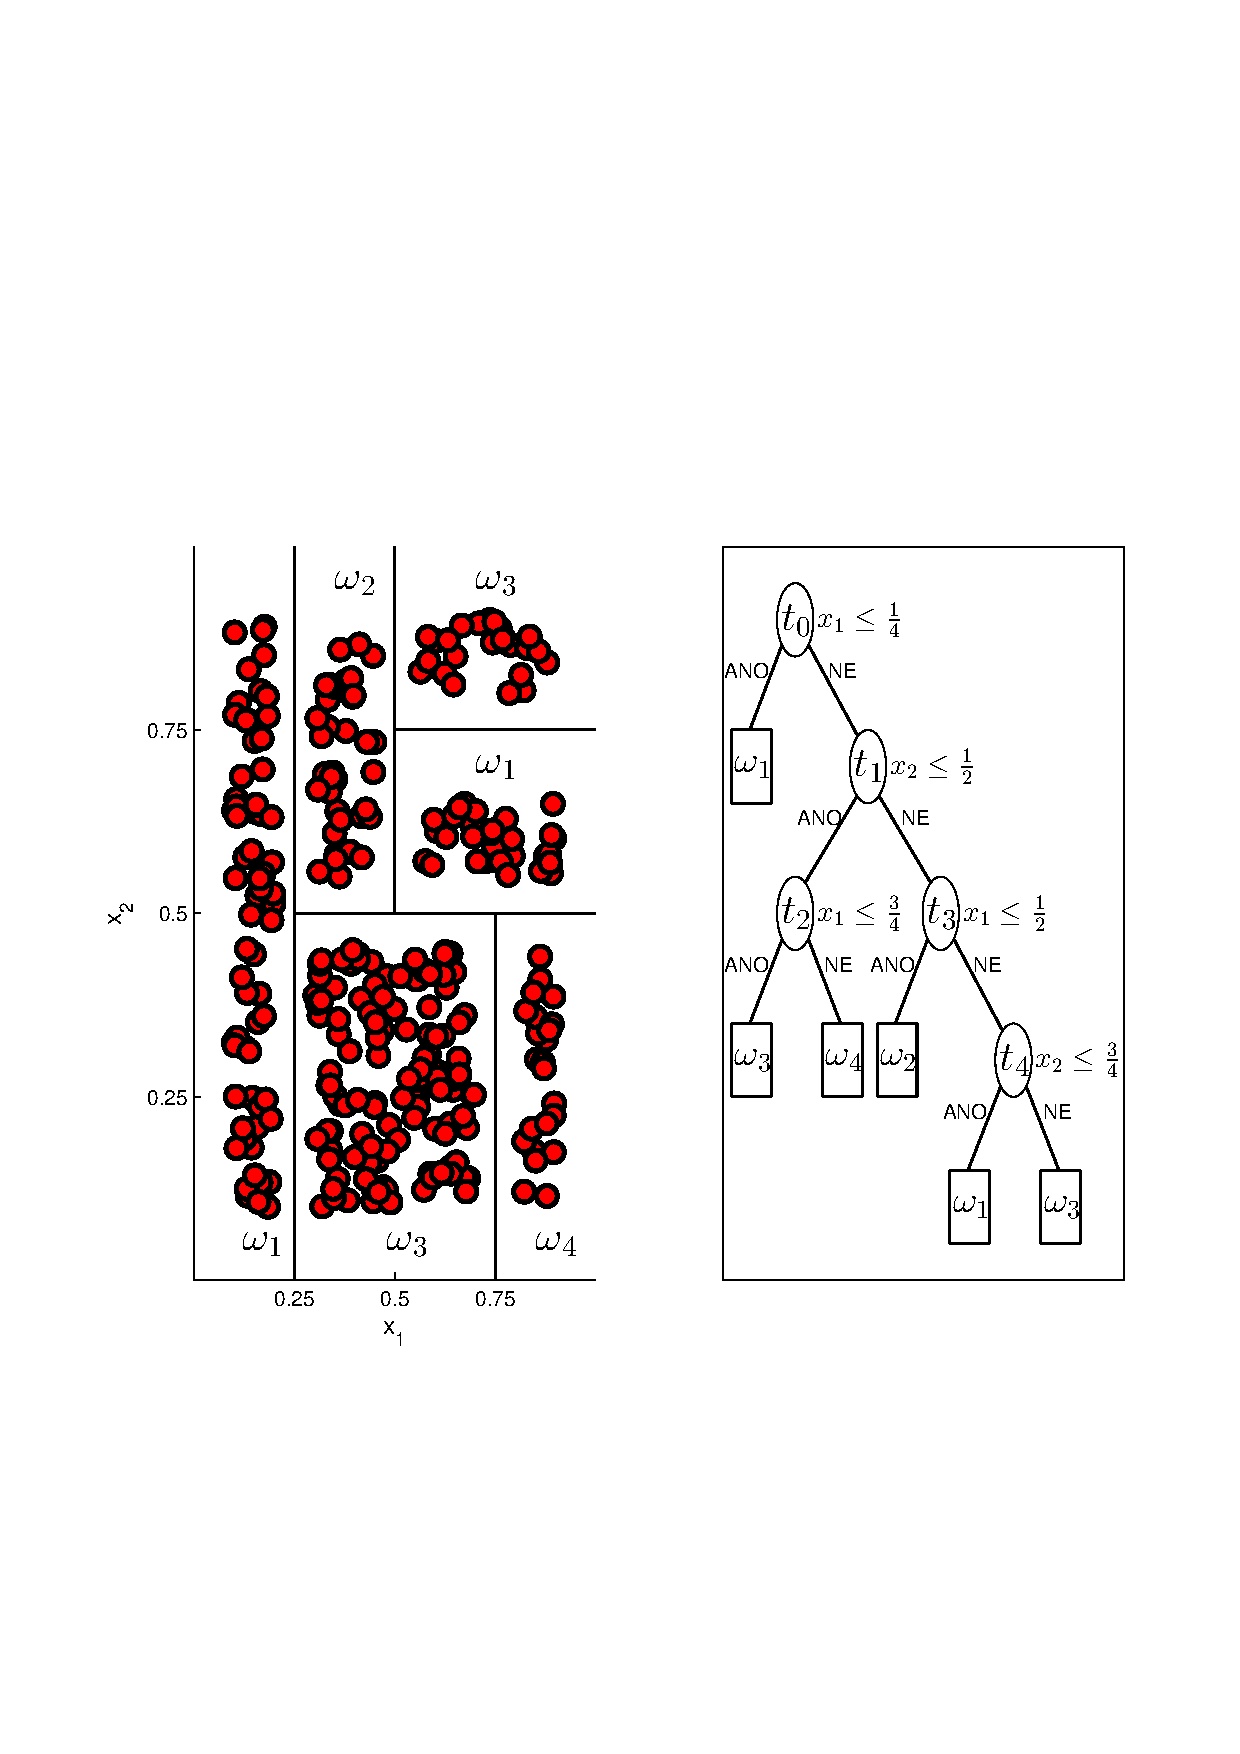
\includegraphics[width = 0.6\textwidth, trim = 3cm 7.5cm 2cm 9cm]{./Img/Prednaska09/decisionTrees/DT01.pdf}
	\caption{Ukázka rozdělení prostoru trénovací množiny (vpravo) pomocí rozhodovacího stromu (vlevo).}
	\label{fig:DT01}
\end{figure}}

\par{Příklad zobrazený na Obr. \ref{fig:DT01} ukazuje princip konstrukce rozhodovacího stromu. Je zřejmé, že výsledný tvar stromu je ovlivněn volbou  rozhodovacího pravidla a pořadím, ve kterém jsou prvky příznakových vektorů porovnávány. Konstrukce každého stromu musí splňovat následující podmínky:
\begin{itemize}
	\item Každý uzel $t$ odpovídá podmnožině $X_t\subset X$, která vznikla na základě rozhodovacího pravidla předešlého uzlu (výjimku tvoří první uzel, tzv. kořen stromu, pro který $X_t=X$). Rozhodovacím pravidlem uzlu $t$ je podmnožina $X_t$ dále rozdělena na $X_{tA}$ a $X_{tN}$. $X_{tA}$ v sobě slučuje vektory, které splnily rozhodovací pravidlo uzlu $t$ a $X_{tN}$ naopak slučuje ty, které pravidlo nesplnily (viz Obr. \ref{fig:DT02}). Každé takové rozdělení musí splňovat:
	\begin{eqnarray}
		\nonumber
		& X_{tA} \cap X_{tN} = \emptyset,\\
		\nonumber
		& X_{tA} \cup X_{tN} = X_t.
	\end{eqnarray}

	\item Ze všech možných rozdělení $X_t$ je zvoleno to, které nejlépe splňuje rozdělující kritérium.
	\item Je nutné zvolit zastavující podmínku, která reguluje narůstání stromu. Uzel, který tuto podmínku splňuje je označena za list stromu.
	\item Každému listu musí být přiřazena odpovídající klasifikační třída.
\end{itemize}
\begin{figure}[!ht]
	\centering
	%trim option's parameter order: left bottom right top
	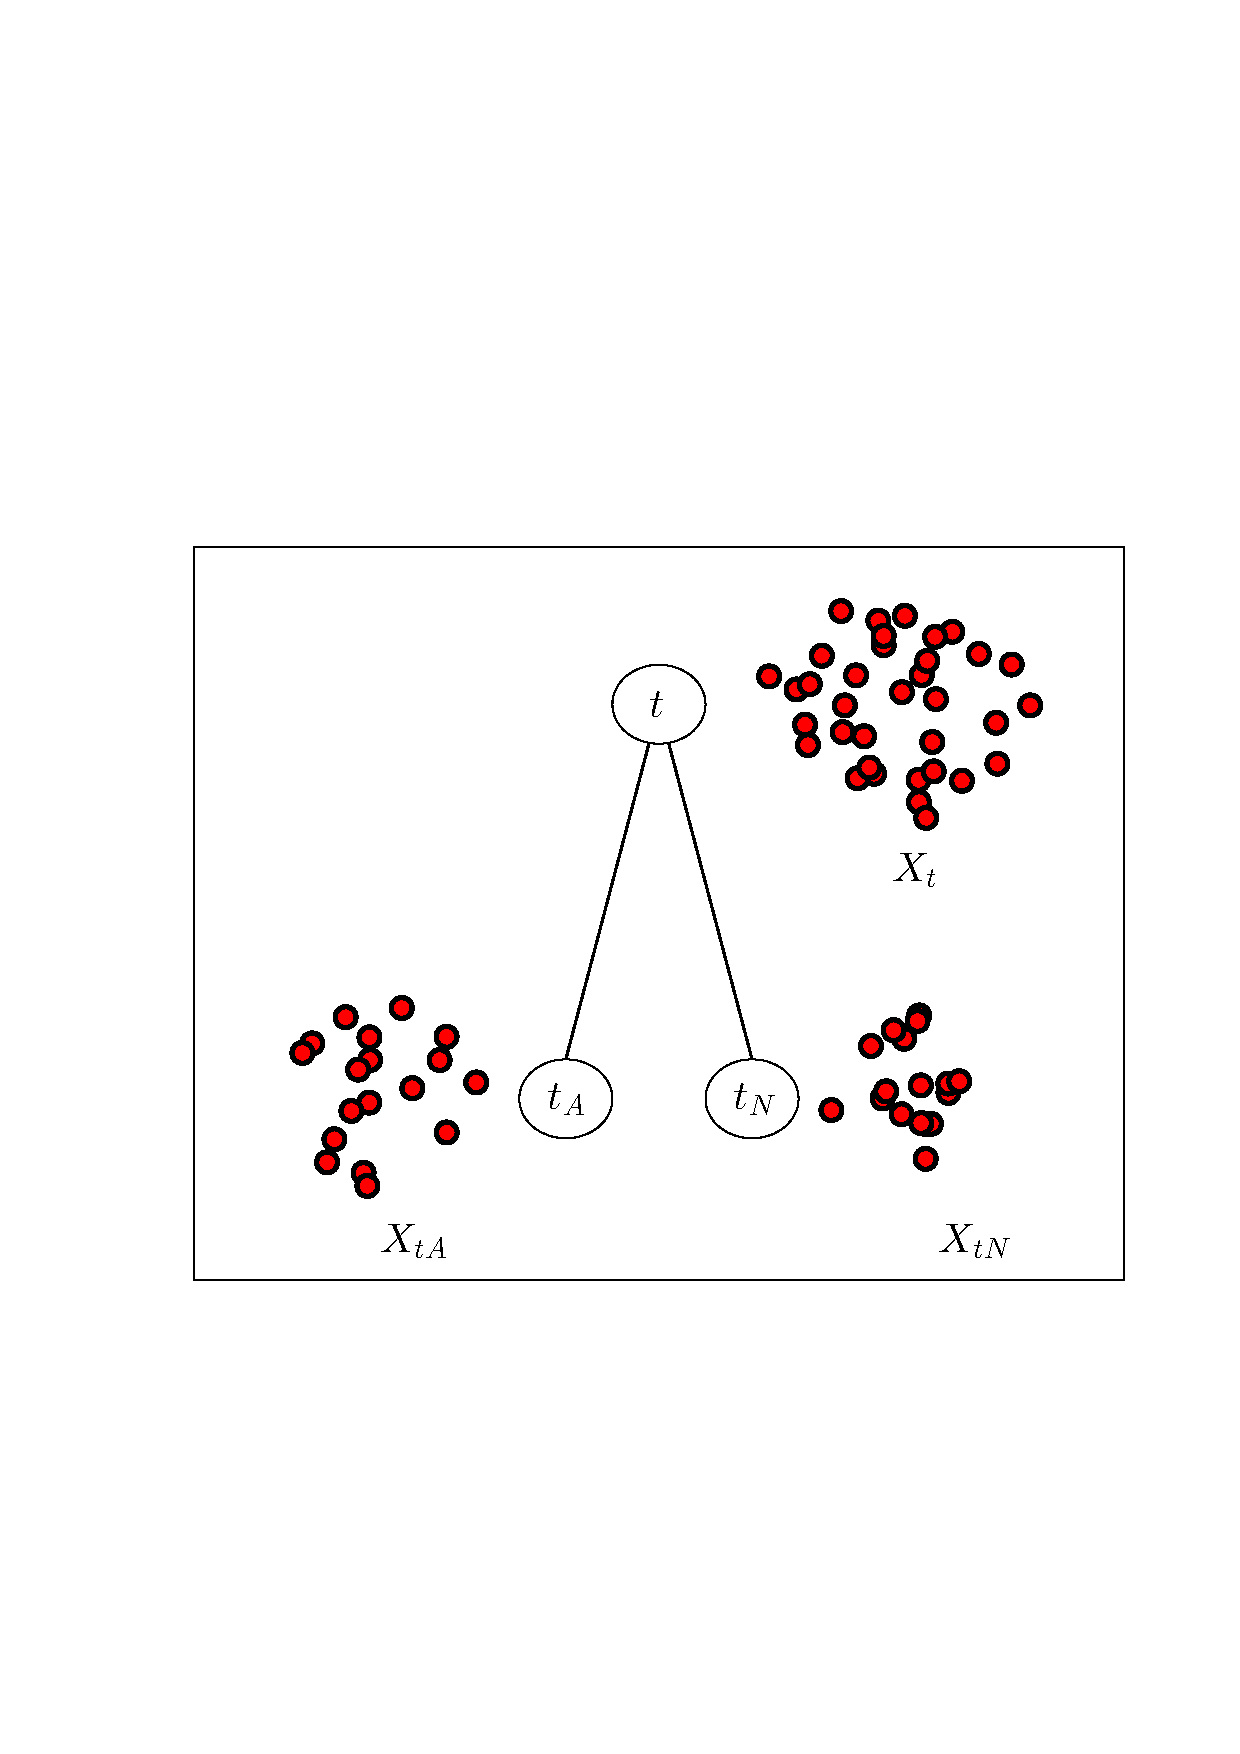
\includegraphics[width = 0.6\textwidth, trim = 3cm 7.5cm 2cm 9cm]{./Img/Prednaska09/decisionTrees/DT02.pdf}
	\caption{Příklad dělení uzlu $t$ a jemu odpovídající množina vektorů $X_t$}
	\label{fig:DT02}
\end{figure}

\par{Pojmy rozdělující kritérium, zastavující podmínka a princip přiřazení klasifikačních tříd listům stromu jsou vysvětleny v následujících podkapitolách.}

\subsection*{Volba rozhodovacího pravidla}
\par{Jak bylo výše uvedeno, v případě binárního stromu má rozhodovací pravidlo tvar $x_i\leq\alpha_i$ ($\alpha_i$ je práh rozdělující vektory na základě porovnání jejich $i$-tého prvku). Úkolem je tedy zvolit jak hodnotu prahu $\alpha_i$, tak i index prvku $i$. Práh však může nabývat nekonečně mnoha hodnot, jelikož $\alpha_i\in\mathrm{R}$ a otestovat všechny z nich je tak nemyslitelné. Díky existenci trénovací množiny $X$ lze ovšem vymezit konečnou množinu hodnot, které je pro získání $\alpha_i$ nutné otestovat. Pokud je porovnáván $i$-tý prvek, $x_i$, vektoru $\bm{x}$, jsou veškeré $i$-té prvky všech příznakových vektorů uvnitř trénovací množiny vzestupně seřazeny a tato řada pak tvoří množinu variant, které je nutné následně podrobit testování. Obdobně se postupuje pro všechny prvky $x_i$,$i=1,2,\ldots ,l$ všech vektorů $\bm{x}\in X$. Postupně tak vznikne několik možností rozdělení podmnožiny $X_t$ a rozdělovacím kritériem je vybráno to nejlepší z~nich. Tímto způsobem je uzlu $t$ určeno, který prvek vektoru $\bm{x}$ se bude uvnitř něj porovnávat s~nalezeným prahem (dojde ke konkretizaci rozhodovacího pravidla $x_i\leq\alpha_i$).}

\subsection*{Rozdělovací kritérium}
\par{Z důvodu, aby bylo možné kvalitativně porovnávat vzniklá rozdělení $X_t$ z předchozího kroku, je definována tzv. míra rozmanitosti uzlu.}

\par{Nechť $P\left(\omega_i\mid t\right)$ značí pravděpodobnost jevu, že vektory uvnitř podmnožiny $X_t$, náležící uzlu $t$, patří do třídy $\omega_i$, $i=1,2,\ldots ,M$. Míra rozmanitosti uzlu je definována jako:
\begin{equation}
	{I\left( t\right) = -\sum_{i=1}^{M} P\left(\omega_i\mid t\right)\log_2 P\left(\omega_i\mid t\right).} \label{eq:entropie}
\end{equation}
Je vhodné poznamenat, že předpis \ref{eq:entropie} představuje entropii z teorie informace spjatou s~uzlem $t$. Ta nabývá svého maxima pokud se všechny pravděpodobnosti $P\left(\omega_i\mid t\right)=\frac{1}{M}$, naopak je rovna nule, pokud všechny vektory uvnitř množiny spadají do jedné třídy,
což znamená, že právě jedna pravděpodobnost $P\left(\omega_i\mid t\right)=1$ a ostatní jsou nulové. V praxi jsou pravděpodobnosti $P\left(\omega_i\mid t\right)$ odhadovány pomocí vztahu $\frac{N_t^i}{N_t}$, kde $N_t^i$ je počet vektorů v $X_t$ patřících do třídy $\omega_i$ a $N_t$ je celkový počet vektorů uvnitř podmnožiny $X_t$.}

\par{Dalším rozdělením $X_t$ na dvě podmnožiny $X_{tA}$ a $X_{tN}$, kde $X_{tA}$ má $N_{tA}$ počet vektorů a $X_{tN}$ má $N_{tN}$ počet vektorů, dojde k nárůstu rozmanitosti uzlu definovaného jako
\begin{equation}
	{\Delta I\left( t\right) = I\left( t\right)-\frac{N_{tA}}{N_t}I\left( t_A\right)-\frac{N_{tN}}{N_t}I\left( t_N\right),}
\end{equation}
kde $I\left( t_A\right)$, $I\left( t_N\right)$ jsou míry rozmanitosti uzlů $t_A$ a $t_N$. Cílem rozdělovacího kritéria tedy  je zvolit takové rozdělení uzlu $t$ (resp. podmnožiny $X_t$), pro které dojde k nejvyššímu nárůstu rozmanitosti uzlu, $\Delta I\left( t\right)$.}

\subsection*{Zastavující podmínka}
\par{Dojde-li k naplnění zastavující podmínky pro některý z uzlů rozhodovacího stromu, je takový uzel prohlášen za list stromu a jeho dělení je ukončeno. Zastavující podmínka může být definována prahem $Tr$, který určuje minimální potřebný nárůst rozmanitosti uzlu, $\Delta I\left( t\right)$. Pokud je po rozdělení uzlu $t$ maximální hodnota $\Delta I\left( t\right)$ přes všechna možná rozdělení uzlu menší než práh $Tr$, je uzel $t$ prohlášen za list. Další možností volby zastavující podmínky je stanovení minimálního počtu vektorů uvnitř podmnožin vzniklých dělením uzlu $t$.}

\subsection*{Princip přiřazení třídy listům}
\par{Jakmile je uzel rozhodovacího stromu prohlášen za list, musí mu být přiřazena jedna z~klasifikačních tříd. Listu je přiřazena třída $\omega_j$, kde index $j$ odpovídá
\begin{equation}
	{j=\mathrm{arg}\min_i P\left(\omega_i\mid t\right).}
\end{equation}
Jinými slovy, listu $t$ je přiřazena taková třída, jenž je uvnitř $X_t$ nejčastěji zastoupena.}

\par{Vedle binárních rozhodovacích stromů lze v odborné literatuře dohledat i stromy, jejichž rozhodovací pravidlo má tvar $\sum_{i=1}^lc_i x_i\leq\alpha$. Jedná se tedy o nalezení přímek, nikoli pouze prahů, dělících jednotlivé prvky příznakových vektorů. Tímto rozhodovacím pravidlem lze sice v některých případe vhodněji rozdělit prostor trénovací množiny $X$, ovšem konstrukce stromu je mnohem složitější.}

\par{Nevýhodou klasifikační metody založené na rozhodovacím stromu zůstává princip sestavování samotného stromu. Pokud dojde byť k malé změně trénovací množiny $X$, dojde zároveň ke změně tvaru rozhodovacího stromu $T$, což může vést k nárůstu chyby klasifikace. Tento nedostatek lze odstranit zapojením více než jednoho rozhodovacího stromu do procesu klasifikace. Taková klasifikační metoda je označována za rozhodovací les.}









\newpage






%----------------------------------------------------------------------------------------
\section{Rozhodovací les}
\label{sec:DecisionWald}
\par{Hlavní předností rozhodovací lesa je to, že účinně potlačuje citlivost výsledného tvaru rozhodovacího stromu $T$ na změny v trénovací množině $X$. Toho je docíleno tak, že množina $X$ obsahující $N$ prvků je algoritmem \textit{bootstrap aggregating} rozdělena na $n$ množin, $X_{\left(n\right)}$, obsahujících $N_{\left(n\right)}$ prvků, přičemž $N_{\left(n\right)}\leq N$. A pro každou množinu $X_{\left(n\right)}$ je následně zkonstruován rozhodovací strom $T_{\left(n\right)}$ postupem, který je popsaný v kapitole \ref{sec:DecisionTree}.}

\par{Klasifikace neznámého vektoru $\bm{y}$ probíhá tak, že je tento vektor přiveden na vstupy všech rozhodovacích stromů $T_{\left(n\right)}$. Každý rozhodovací strom poté určí příslušnost vektoru $\bm{y}$ do některé třídy $\omega_i$, $i=1,2,\ldots ,M$. Finální index třídy $i$ je vybrán na základě nejčastějšího výsledku mezi všemi provedenými klasifikacemi (tj. výstupy stromů $T_{\left(n\right)}$) neznámého vektoru $\bm{y}$.}

\par{Dalším faktorem, jenž ovlivňuje výsledný tvar rozhodovacího stromu, je pořadí prvků příznakových vektorů, které je během nalézání rozhodovacích pravidel pro jednotlivé uzly uvažováno. Doposud byly v tomto textu představeny rozhodovací stromy využívající
ke své konstrukci prvky vektorů popořadě. Následující kapitola popisuje modifikaci rozhodovacích lesů, jež stanoví toto pořadí náhodně.}



















%----------------------------------------------------------------------------------------
\section{Náhodný les}
\label{sec:RandomWald}
\par{Náhodný les je modifikací metody rozhodovacího lesa, která vznikla
za účelem ještě většího zpřesnění výsledku klasifikace. Jsou-li během konstrukce stromů porovnávány prvky příznakových vektorů popořadě, zvyšuje se tím riziko toho, že velká část takto vzniklých stromů bude vzájemně korelovaná. Ovšem vysoká korelace stromů, jak bylo prokázáno, uvnitř rozhodovacího lesa zvyšuje chybu klasifikace. Z tohoto důvodu používá náhodný les zcela nový princip konstrukce jednotlivých rozhodovacích stromů.}
\par{Prvním krokem této metody zůstává rozdělení trénovací množiny $X$ na $n$ množin pomocí algoritmu \textit{bootstrap aggregating}. Rozdíl nastává v bodě konstrukce jednotlivých stromů. Během té je nejprve uživatelem zvolen parametr $m$ ($m<<l$, kde $l$ je dimenze vektoru $\bm{x}\in X$),
který ovlivňuje volbu rozhodovacího pravidla pro jednotlivé uzly konstruovaných stromů. Jako rozhodovací pravidlo je totiž zvoleno to, které vykáže nejlepší výsledek mezi $m$ náhodně vybranými prvky příznakového vektoru. Tímto způsobem vznikají všechny stromy tvoří finální náhodný les. Klasifikace neznámého vektoru $\bm{y}$ pak probíhá stejně, jako tomu bylo v případě klasického rozhodovacího lesa.
}









\newpage





%----NEURONOVE-SITE--------------------------------------------------------------------
\section{Neuronové sítě}
\par{Dříve popsaná klasifikační metoda SVM usiluje o nalezení takové nadroviny $g\left(x\right)$, která rozděluje trénovací množinu $X$ do dvou tříd $\omega_1$, $omega_2$. V případě lineárně separovatelné množiny nalezená nadrovina $g\left(x\right)$ klasifikovala trénovací vektory, $\bm{x}\in X$, bez chyby. Pokud ovšem trénovací množina lineárně separovatelná nebyla, cílem metody SVM bylo zkonstruovat nadrovinu $g\left(x\right)$ minimalizující chybu klasifikace. Klasifikátory pracující na~principu neuronových sítí byly primárně navrženy právě k řešení lineárně neseparovatelných problémů. Řešení je nalezeno pomocí transformace těchto problémů
do prostoru, ve~kterém již existuje adekvátní lineární řešení.}

\par{Základním stavebním kamenem neuronové sítě je neuron, na jehož vstup je přiveden vektor $\bm{x}$ a výstupem je pak 1 (je-li $\bm{x}\in\omega_1$)  či 0 (je-li $\bm{x}\in\omega_2$). Neuron s takovýmto binárním výstupem je označován jako perceptron. Neuronová síť, skládající se výhradně z perceptronů, se nazývá perceptronová síť a pokud v ní dochází k řazení perceptronů za sebe, je taková síť označována jako vícevrstvá perceptronová síť (MLP - \textit{Multilayer perceptron}). Princip fungování MLP bude popsán v následující části textu na příkladu dvouvrstvé perceptronové sítě.}

\subsection*{Dvouvrstvá perceptronová síť}
\par{Úkolem této neuronové sítě je klasifikovat $l$-dimenzionální vektor $\bm{x}\in\mathcal{R}^l$ pomocí $p$ perceptronů (viz Obr. \ref{fig:NN01}a). Tyto perceptrony se nacházejí v tzv. skryté vrstvě a jejich úkolem je namapovat $l$-dimenzionální vstupní vektor do $p$-dimenzionálního prostoru $H_p$, který si lze představit jako vrcholy prostorového mnohoúhelníku definovaného:
\begin{displaymath}
	H_p=\{\left[y_1,\ldots,y_p\right]^\top\in\mathcal{R}^p,y_i\in\{0,1\},1\leq i \leq p \}.
\end{displaymath}
Každý perceptron ve skryté vrstvě sítě vlastně představuje jednu klasifikační nadrovinu
a~převádí lineárně neseparovatelnou trénovací množinu $X$ do prostoru, v němž je ji možné bez chyby rozdělit do dvou tříd (viz Obr. \ref{fig:NN01}b).







\newpage











\begin{figure}[!ht]
	\centering
	%trim option's parameter order: left bottom right top
	%\fbox{
	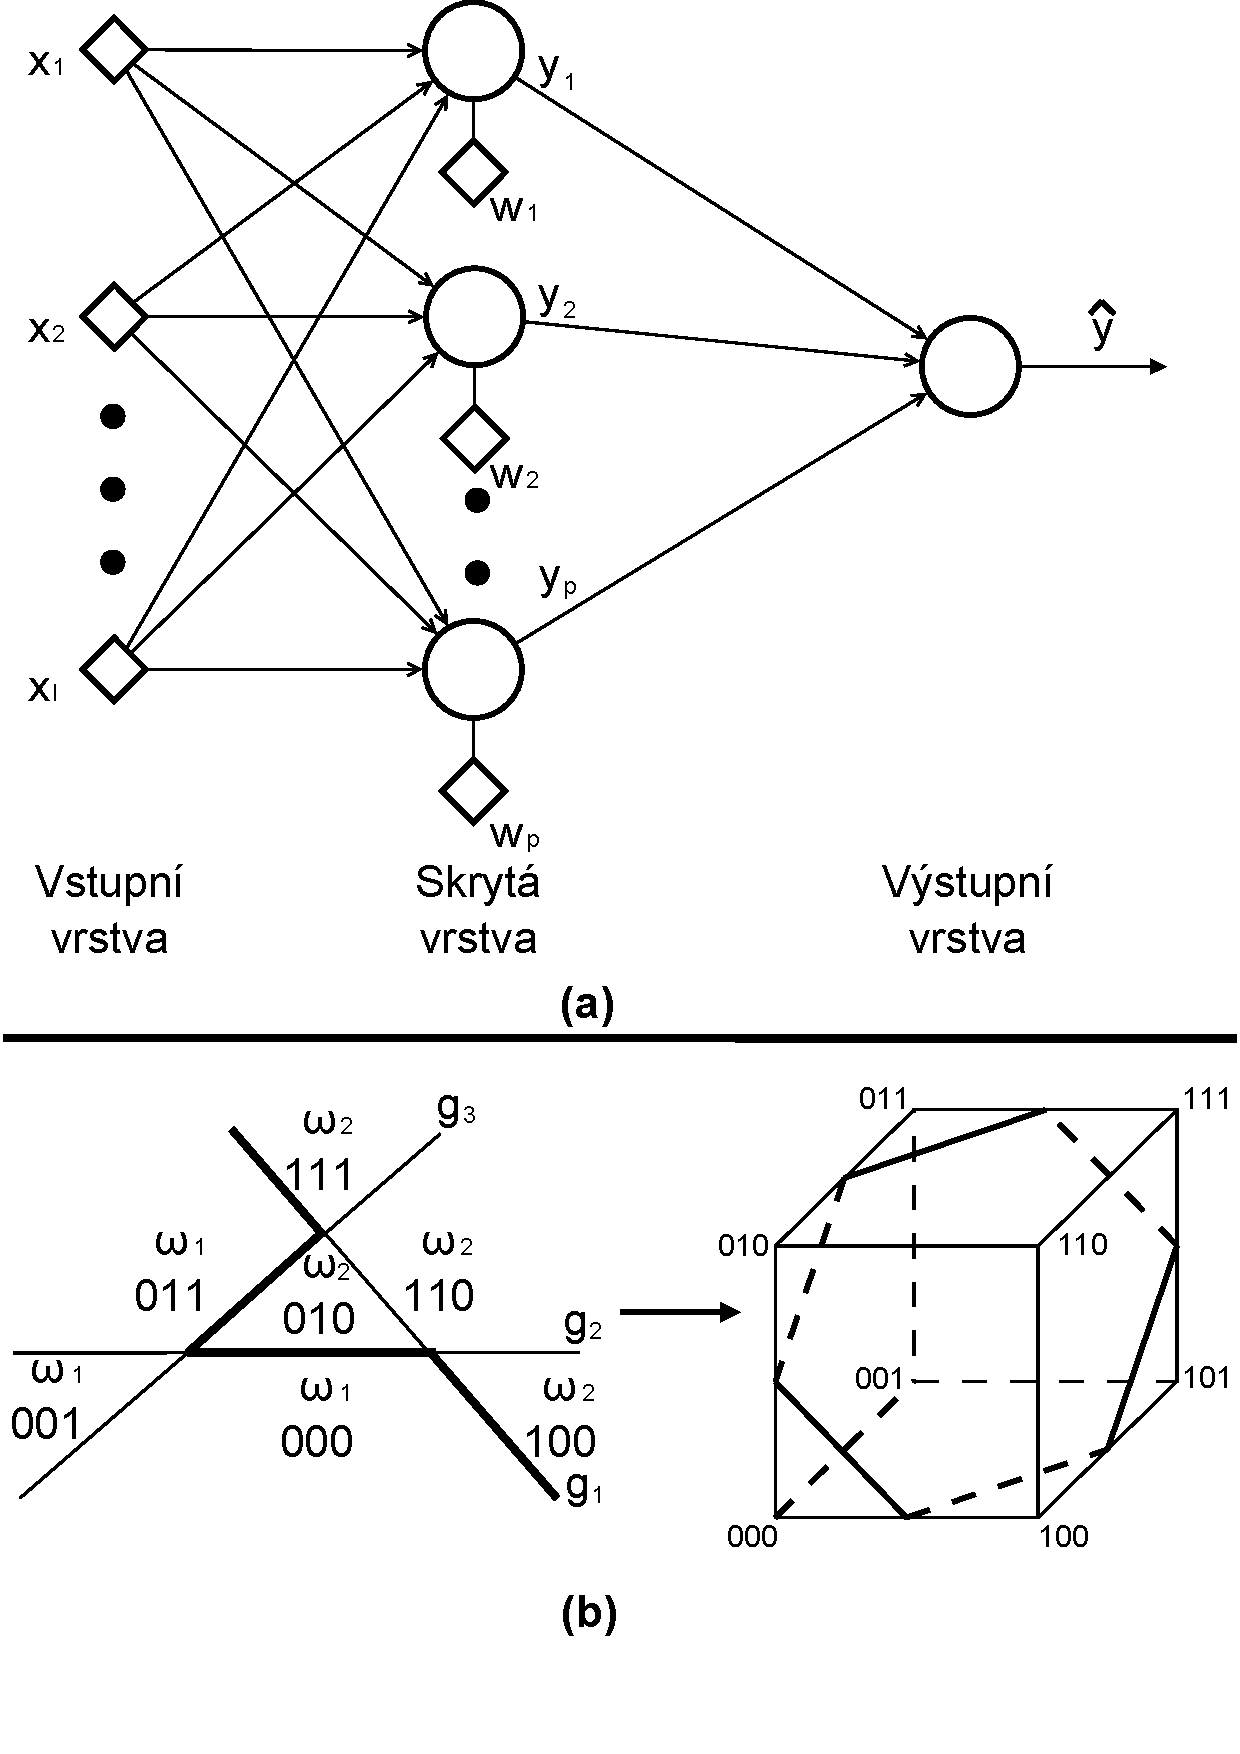
\includegraphics[width = 0.6\textwidth, trim = 0cm 2cm 0cm 0cm]{./Img/Prednaska09/nn/NN01.pdf}
	\caption{(a) Dvouvrstvá perceptronová síť, (b) Příklad transformace nelineárně separovatelného problému do prostoru, ve kterém existuje lineární řešení; neuronová síť je tvořena třemi perceptrony ve skryté vrstvě (perceptrony představují klasifikační nadroviny $g_1,g_2,g_3$).}
	\label{fig:NN01}
\end{figure}}

\par{Vícevrstvé perceptronové sítě se používají v případě komplikovanějších klasifikačních úloh. Jejich konstrukce obsahuje více skrytých vrstev a pracují na principu rozložení složitého problému na menší mnohem jednodušší problémy. Kombinací řešení těchto dílčích problémů je následně dosaženo hledaného výsledku}





\newpage





\subsection*{Aktivační funkce}
\par{Uvažujme jednoduchý perceptron s dvěma vstupy  $x_1$, $x_2$ a jedním výstupem $y$ (viz Obr. \ref{fig:NN02}). Výstup takového perceptronu odpovídá předpisu:
\begin{figure}[!ht]
	\centering
	%trim option's parameter order: left bottom right top
	%\fbox{
	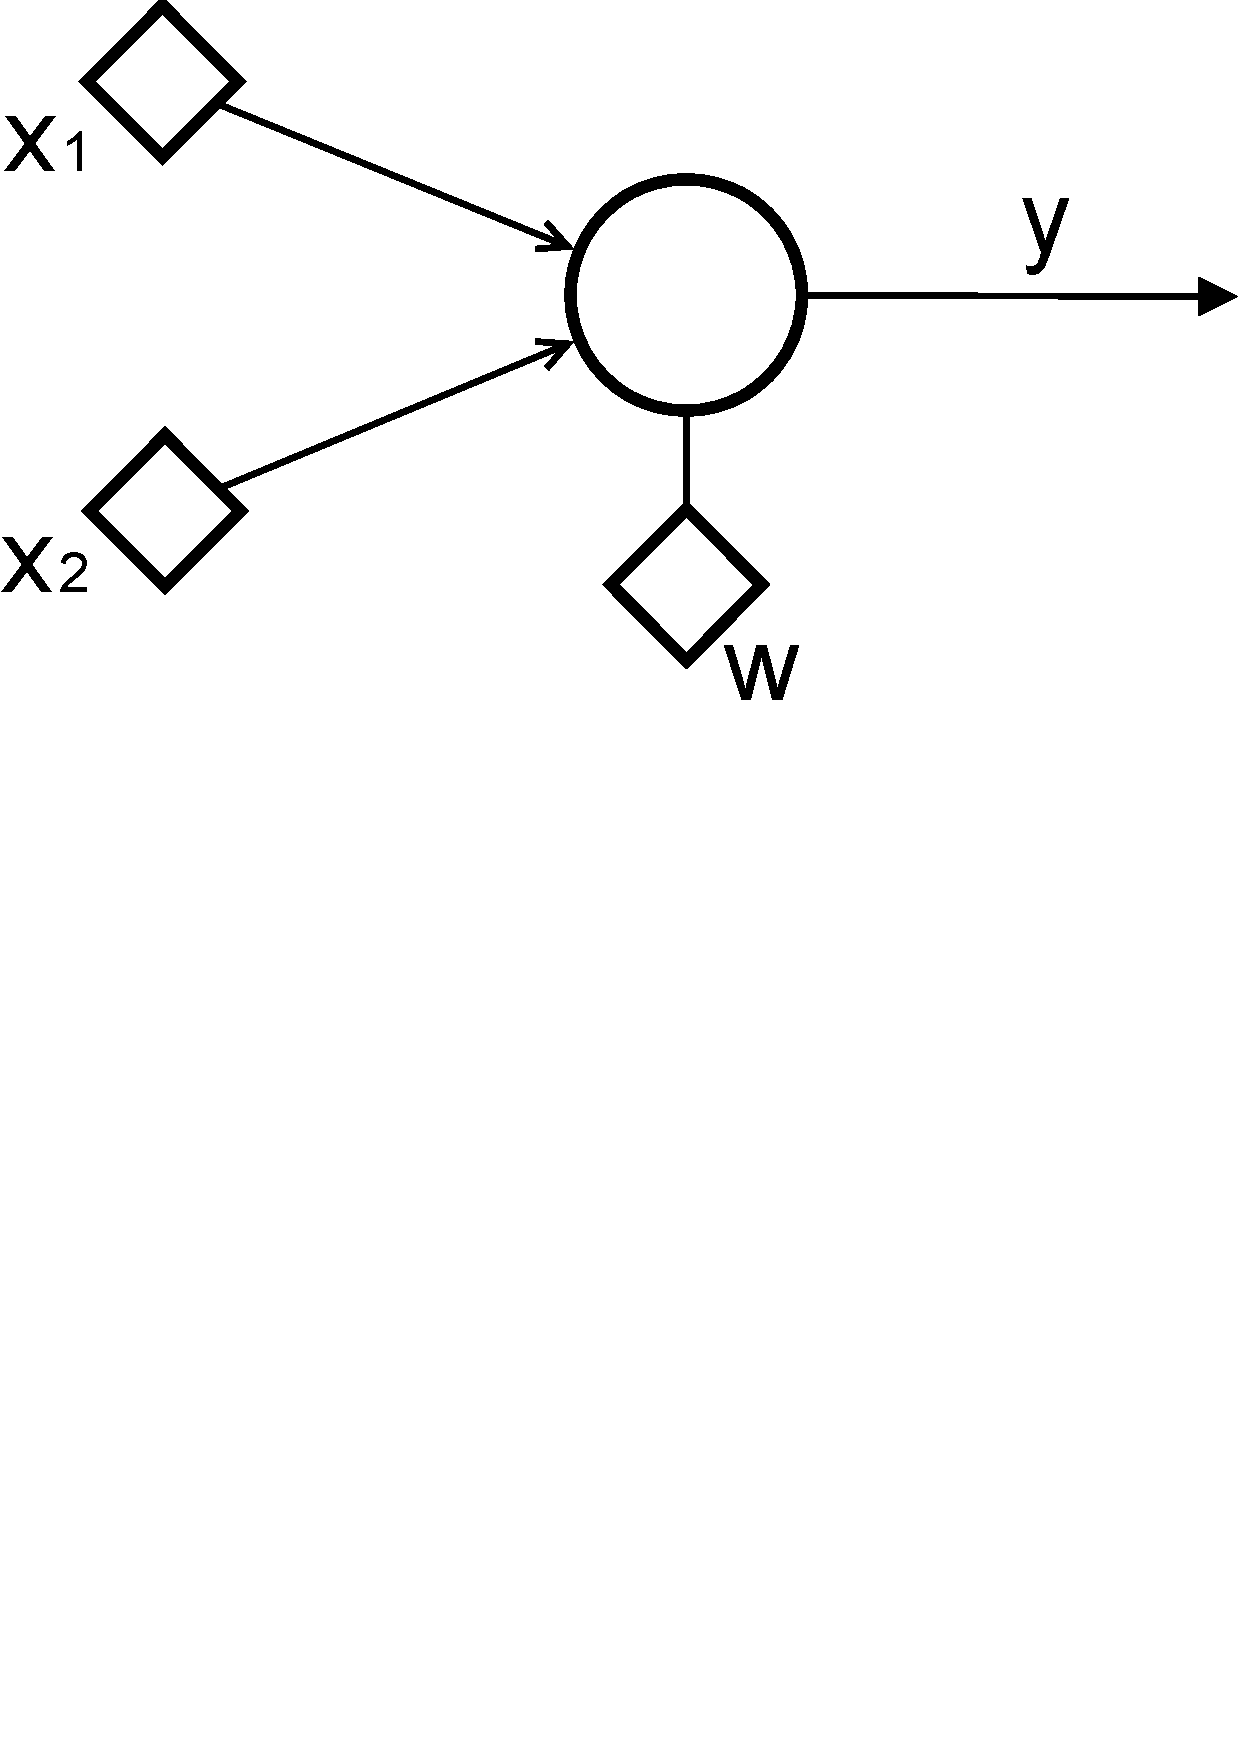
\includegraphics[width = 0.4\textwidth, trim = 0cm 18cm 0cm 0cm]{./Img/Prednaska09/nn/NN02.pdf}
	\caption{Perceptron.}
	\label{fig:NN02}
\end{figure}
\begin{displaymath}
	y=f\left(a\right)\text{, kde }~a=\sum_{i=1}^2\left(wx_i\right).
\end{displaymath}
Funkce $f\left(a\right)$ je označována jako aktivační funkce neuronu a $w$ je jeho synaptická váha. Mezi nejčastěji používané aktivační funkce patří:
\begin{itemize}
	\item Skoková funkce
		\begin{equation}
			f\left(a\right)=\left\{
			\begin{array}{ll}
				1 & \text{pro}~a>0 \\
				0 & \text{pro}~a<0
			\end{array} \right.
		\end{equation}
	\item Sigmoida
		\begin{equation}
			f\left(a\right)=\frac{1}{1+\mathrm{exp}\left(-\lambda a\right)}
		\end{equation}
		kde $\lambda$ je parametr sklonu.
	\item Hyperbolický tangens
		\begin{equation}
			f\left(a\right)=\frac{1+\mathrm{exp}\left(-\lambda a\right)}{1-\mathrm{exp}\left(-\lambda a\right)}
		\end{equation}
\end{itemize}}

\par{Proces trénování neuronové sítě spočívá v nastavení synaptických vah jednotlivých neuronů. Jelikož je k dispozici trénovací množina jedná se opět o tzv. učení s učitelem, které je realizováno např. algoritmem zpětného šíření (\textit{Backpropagation Algorithm}).}

\subsection*{Algoritmus zpětného šíření}
\par{Algoritmus vychází z trénovací množiny, která obsahuje $N$ dvojic ($y\left( i\right)$, $\bm{x}\left( i\right))$, pro $i = 1, 2, \ldots, N$, kde $\bm{x}\left( i\right)$ představuje $i$-tý vektor trénovací množiny a $y\left( i\right)$ určuje jeho příslušnost do jedné ze tříd. Během trénování jsou v jednotlivých iteracích získávány výstupy neuronové sítě $\hat{y}\left( i\right)$,
které se liší od požadovaného $y\left( i\right)$. Cílem učení je nastavit synaptické váhy jednotlivých vrstev sítě tak, aby rozdíl mezi aktuálním výstupem $\hat{y}\left( i\right)$ a požadovaným výstupem $y\left( i\right)$ byl minimální.}

\par{Nové synaptické váhy jsou vypočítávány jako
\begin{equation}
	w_j^r\left(nova\right)=w_j^r\left(stara\right)+\Delta w_j^r, \label{eq:aktWei}
\end{equation}
kde $w_j^r$ je váha $j$-tého neuronu v $r$-té vrstvě sítě a $\Delta w_j^r$ značí přírůstek, který je definován
\begin{equation}
	\Delta w_j^r=-\mu\frac{\partial J}{\partial w_j^r},
\end{equation}
kde $\mu$ je konstanta učení (parametr algoritmu). Cílem algoritmu zpětného šíření je minimalizace nákladové funkce $J$ s předpisem:
\begin{equation}
	J=\sum_{i=1}^N\mathcal{E}\left(i\right), \label{eq:energyJ}
\end{equation}
kde lze za $\mathcal{E}\left(i\right)$ zvolit rozdíl čtverců
\begin{equation}
	\mathcal{E}\left(i\right)=\frac{1}{2}\sum_{i=1}^N\left(y\left(i\right)-\hat{y}\left(i\right)\right)^2.
\end{equation}
Přírůstek $\Delta w_j^r$ ze vzorce \ref{eq:aktWei} je stanoven vyřešením rovnice
\begin{equation}
	\frac{\partial \mathcal{E}\left(i\right)}{\partial w_j^r}=0. \label{eq:grad}
\end{equation}}

\par{Algoritmus učení neuronové sítě probíhá v několika krocích. Nejprve jsou náhodně
nastaveny synaptické váhy $w_j^r$ pro jednotlivé neurony (obvykle se doporučuje váhy volit
v~intervalu $\left\langle-1,1\right\rangle$) a je zvolena hodnota konstanty učení $\mu>0$ a maximální chyby $\mathcal{E}_{max}>0$. Tento krok se nazývá inicializace. Poté je spočtena odezva vstupního vektoru $\hat{y}\left(i\right)$ a dojde k aktualizaci vah podle vzorce \ref{eq:aktWei}. Obdobně se postupuje pro všechny prvky $x\left(i\right)\in X$ z~trénovací množiny. Jestliže je na konci trénovacího cyklu výsledná chyba $\sum_{i=1}^N\mathcal{E}\left(i\right)\leq\mathcal{E}_{max}$ algoritmus skončí, v opačném případě dojde k nové inicializaci plynoucí z řešení rovnice \ref{eq:grad} a algoritmus se zopakuje.}

\par{Algoritmus zpětného šíření představuje jednoduchý způsob učení neuronové sítě,
který ovšem velmi kvalitně vystihuje princip takového učení. V odborné literatuře 
se lze setkat i se složitějšími algoritmy učení, mezi které patří algoritmy založené
na určení směru gradientu funkce \ref{eq:energyJ} či algoritmy využívající kvazi-Newtonovu metodu.}











\newpage









%----KONVOLUCNI-SITE-------------------------------------------------------------------------
\section{Konvoluční neuronové sítě}
\par{Za účelem klasifikace obrazových dat jsou momentálně v praxi nejhojněji využívány tzv.~konvoluční neuronové sítě (CNN - \textit{Convolutional Neural Networks}), které mají podobnou strukturu jako běžné neuronové sítě, ale výstupy jednotlivých vrstev nejsou získávány pomocí aktivační funkce neuronů, nýbrž pomocí konvoluce vstupu a příslušného konvolučního jádra.}

\par{CNN se od klasické neuronové sítě liší již svým vstupem. Vstupem totiž není příznakový vektor obrazu, ale obraz samotný (viz Obr. \ref{fig:CNN01}). Nad vstupním obrazem je provedena konvoluce, jejíž výsledek představuje výstup konvoluční vrstvy. Ta může být následována vrstvou max-poolingu, nebo další konvoluční vrstvou. Konvoluce probíhá pouze nad~definovaným prostorem vstupu, tzn. že konvoluční jádro nesmí zasahovat mimo okraje vstupního obrazu. Zřetězením těchto operací je postupně redukována velikost vstupního obrazu až do bodu, kdy je výstupem pouze jednodimenzionální příznakový vektor. Ten je v nejvyšší vrstvě sítě (v tzv. klasifikační vrstvě) zařazen do jedné klasifikační třídy.
\begin{figure}[!ht]
	\centering
	%trim option's parameter order: left bottom right top
	%\fbox{
	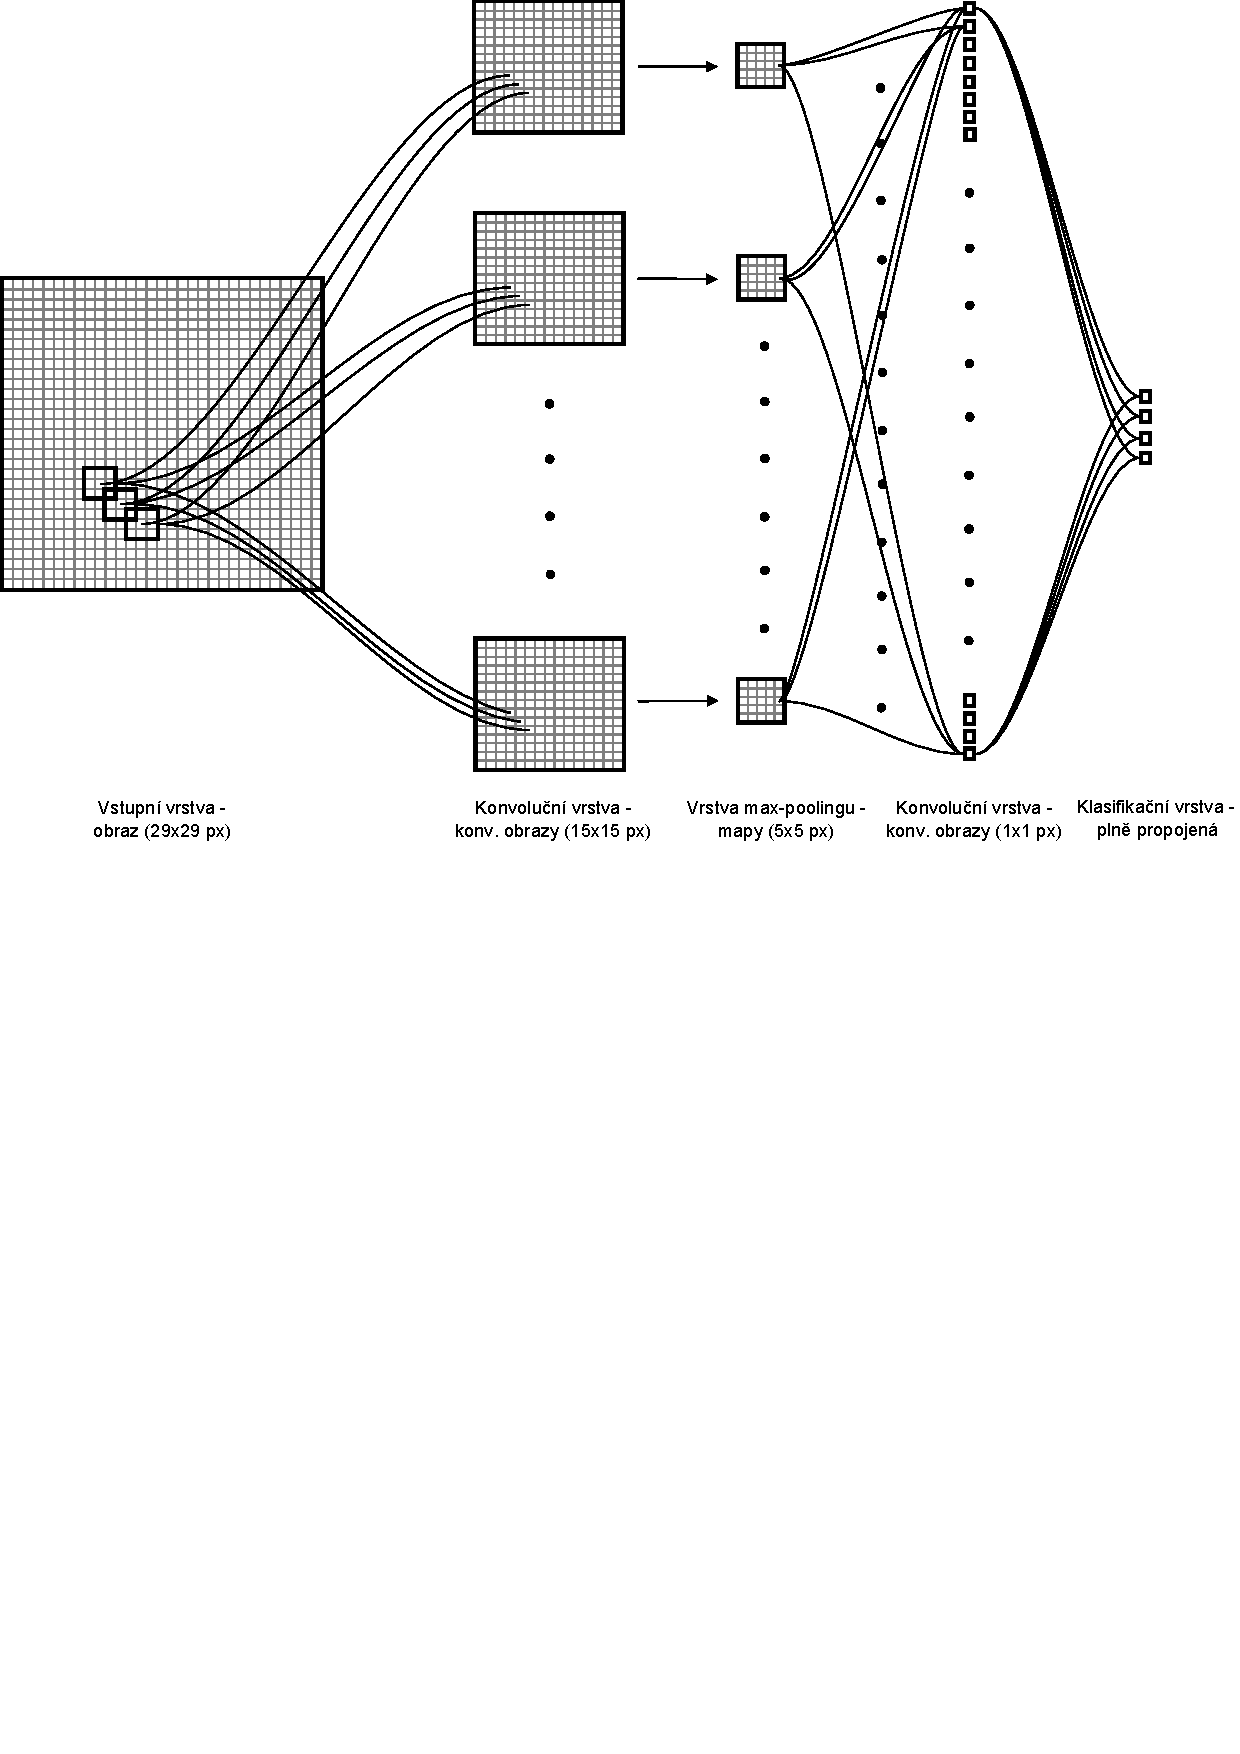
\includegraphics[width = 1\textwidth, trim = 0cm 15cm 0cm 0cm]{./Img/Prednaska09/cnn/CNN01.pdf}
	\caption{Architektura konvoluční neuronové sítě; velikost konvolučních jader je $3\times 3$, hodnota posunu je nastavena na $1$ a klasifikace probíhá do čtyř tříd.}
	\label{fig:CNN01}
\end{figure}}

\subsection*{Konvoluční vrstva}
\par{Konvoluční vrstva je určena počtem a velikostí konvolučních jader a hodnotou posunu. Počet konvolučních jader $M$ určuje počet výstupů vrstvy, které posléze vstupují do vrstvy následující. Hodnota posunu, $S_x$ a $S_y$, definuje o kolik pixelů se jádro během konvoluce po vstupním obraze posouvá ve směru osy $x$ a $y$. Velikost konvolučního jádra ($K_x$, $K_y$) spolu s hodnotou posunu určují velikost výstupních konvolučních obrazů ($M_x$, $M_y$).}

\subsection*{Vrstva max-poolingu}
\par{Max-pooling představuje proces podvzorkování vstupního konvolučního obrazu. Tento proces je do CNN zařazen z důvodu, že urychluje konvergenci sítě a vede k nalezení robustnějších obrazových příznaků. Max-pooling pracuje na principu detekce maxim v~nepřekrývajících se regionech vstupního obrazu. Tyto regiony jsou definovány velikostí konvolučního jádra ($K_x$, $K_y$). Výstupem vrstvy max-poolingu je tedy mapa obsahující nalezená maxima a rozměr mapy odpovídá podvzorkování vstupního obrazu o faktor $K_x$, resp. $K_y$, podél obou os (viz Obr. \ref{fig:CNN02}).
\begin{figure}[!ht]
	\centering
	%trim option's parameter order: left bottom right top
	%\fbox{
	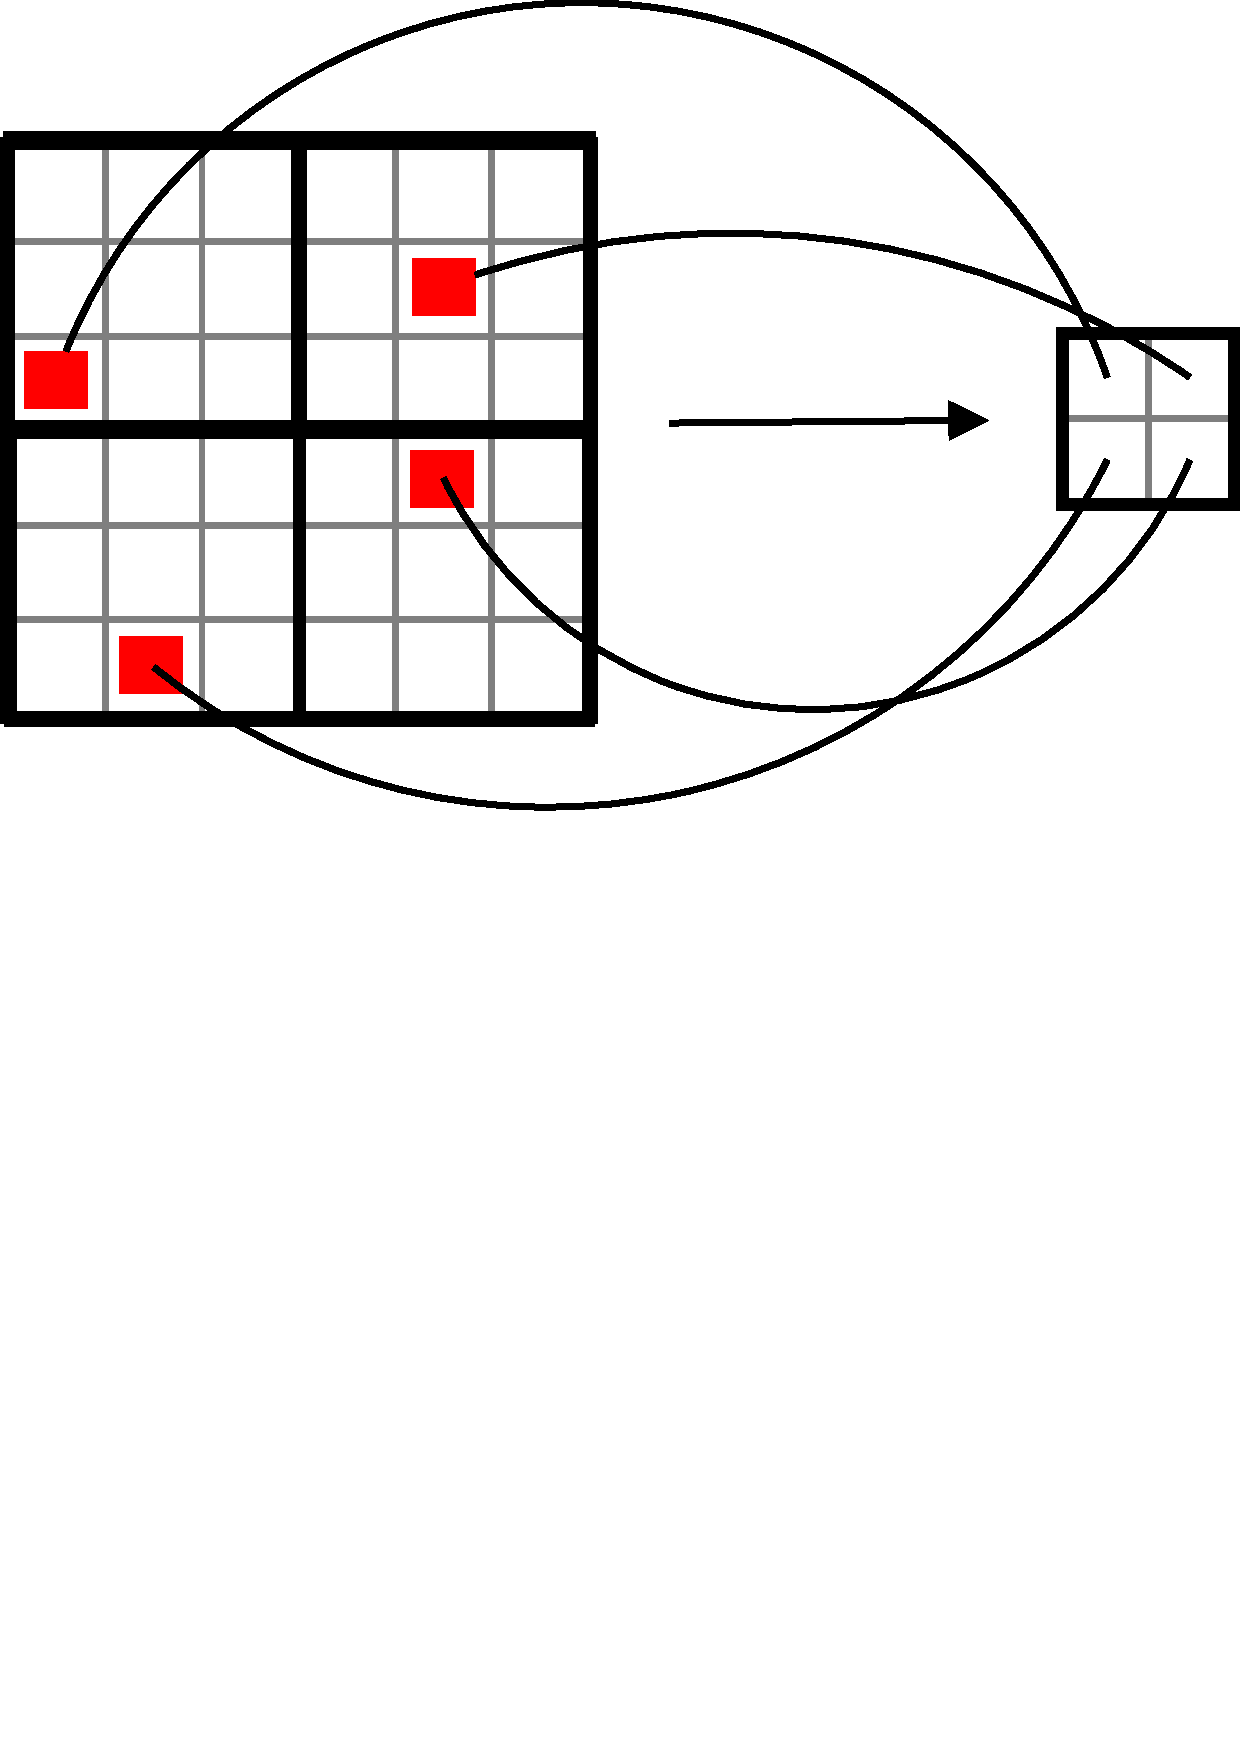
\includegraphics[width = 0.6\textwidth, trim = 0cm 15cm 0cm 0cm]{./Img/Prednaska09/cnn/CNN02.pdf}
	\caption{Ukázka max-poolingu; maxima dílčích regionů vstupního obrazu jsou vyznačena červeně a regiony mají rozměr $3\times 3$.}
	\label{fig:CNN02}
\end{figure}}

\subsection*{Klasifikační vrstva}
\par{Tato vrstva představuje nejvyšší vrstvu CNN a obsahuje přesně tolik neuronů, kolik je klasifikačních tříd. Bývá také označována jako plně propojená vrstva, jelikož na vstup každého jejího neuronu jsou přivedeny všechny výstupní konvoluční obrazy vrstvy předešlé. Jak již bylo poznamenáno, výstupy předcházející vrstvy představují jednodimenzionální příznakový vektor vstupního obrazu, u kterého je následně rozhodnuto, do jaké náleží třídy.}

\par{Učení CNN probíhá obdobným způsobem jako učení klasické neuronové sítě. Jen s~tím rozdílem, že nedochází k aktualizaci vah, ale jsou upravovány formy jednotlivých konvolučních jader.}









\newpage

\section{Zdroje}

\label{sec:08_References}
\par{$\left[1\right]$	Richard O. Duda, Peter E. Hart, David G. Stork, , \textit{Pattern Classification (2nd Edition)}, Wiley-Interscience, 2000.}
\newline
$\left[2\right]$	Breiman L., \uv{Bagging Predictors}, \textit{Machine Learning}, Vol. 24, pp. 123-140, 1996.\newline
$\left[3\right]$	Breiman L., \uv{Random Forests}, \textit{Machine Learning}, Vol. 45, pp. 5-32, 2001.\newline
$\left[4\right]$	Quinlan J.R., \textit{C4.5: Programs for Machine Learning}, Morgan Kaufmann, 1993.\newline
$\left[5\right]$	Theodoridis S., Koutroubas K., \textit{Pattern Recognition}, Elsevier Inc., 2008.}















\end{document}

